\documentclass[11pt,a4paper]{article}

\usepackage[utf8]{inputenc}
\usepackage[T1]{fontenc}
\usepackage[brazil]{babel}
\usepackage{lmodern}
\usepackage[margin=2.5cm]{geometry}
\usepackage{amsmath}
\usepackage{graphicx}
\usepackage{booktabs}
\usepackage[font=small,labelfont=bf]{caption}
\usepackage[authoryear,round]{natbib}
\usepackage[hidelinks]{hyperref}

\title{Previsão de curto prazo do consumo residencial de energia elétrica\\com redes neurais}
\author{Ian Teixeira Barreiro (10717526) \and Ornella Scardua Ferreira (\textbf{[NUSP]})\\[4pt]
\small MAE5920 -- Deep Learning, IME-USP. Prof.\ Dr.\ Hamed Yazdanpanah}
\date{Novembro de 2026}

\begin{document}
\maketitle

\begin{abstract}
Prevemos o consumo dos eletrodomésticos de uma casa, a cada 10 minutos, com horizontes de 10 e 60 minutos. Comparamos a persistência, um modelo autorregressivo com variáveis exógenas (ARX), um MLP, uma CNN 1D e uma GRU, todos avaliados nas mesmas origens de previsão. Na primeira rodada, as redes que previam o nível do consumo foram bem na validação e falharam no teste, por uma mudança na distribuição das entradas: o período de teste é muito mais quente que o de treino. Uma cabeça residual, que faz a rede partir da persistência, resolveu o problema. Com ela, a GRU teve MAE de teste de 23,7 e 35,0~Wh, contra 27,1 e 40,3~Wh do ARX. Os picos de consumo continuam sendo o principal modo de falha de todos os modelos, inclusive de um modelo de fundação (Chronos-2) avaliado como extra.
\end{abstract}

% ===========================================================================
\section{Introdução}

Previsões de consumo com antecedência de minutos a uma hora são úteis para o gerenciamento de carga e para sistemas domésticos de controle. Usamos a base \emph{Appliances Energy Prediction} \citep{candanedo2017} e prevemos o consumo dos eletrodomésticos com horizontes de 10 e 60 minutos. Comparamos duas referências (persistência e ARX) com três redes neurais (MLP, CNN 1D e GRU). Todas usam a mesma divisão temporal e são avaliadas nas mesmas origens.

O trabalho teve duas rodadas. Na rodada~1, as redes perderam para a persistência e para o ARX no teste, apesar de bons resultados na validação. O diagnóstico foi uma mudança na distribuição das entradas (\emph{covariate shift}). Em resposta, mudamos o \emph{protocolo de seleção de modelos} para uma validação com janelas expansivas, com regras de decisão fixadas antes dos resultados, e introduzimos uma cabeça residual. A divisão em treino, validação e teste não mudou. Como a rodada~2 foi motivada pelo resultado de teste da rodada~1, reportamos as duas rodadas e discutimos essa limitação na Seção~\ref{sec:falha}.

% ===========================================================================
\section{Dados e análise exploratória}

A base tem 19\,735 observações a cada 10 minutos, de 11/01/2016 17h00 a 27/05/2016 18h00, sem lacunas nem valores faltantes. Além do consumo dos eletrodomésticos (\texttt{Appliances}, em Wh), há o consumo das luzes e a temperatura e a umidade de nove sensores: oito cômodos e um do lado de fora do prédio (\texttt{T6}, \texttt{RH\_6}). Há também seis variáveis meteorológicas da estação de Chièvres e duas variáveis aleatórias (\texttt{rv1}, \texttt{rv2}), incluídas pelos autores para testar seleção de variáveis.

O consumo é muito assimétrico (Figura~\ref{fig:eda}b): a mediana é 60~Wh, a média é 98~Wh, o percentil~95 é 330~Wh e o máximo é 1\,080~Wh. O perfil diário (Figura~\ref{fig:eda}a) é baixo de madrugada, sobe pela manhã e tem um pico às 18h em todos os dias da semana. Segundas e sextas têm consumo alto à tarde, talvez por trabalho em casa, e terças, quartas, quintas e domingos têm tardes mais calmas. Esse padrão diário e semanal motivou as variáveis de calendário.

Entre as demais variáveis, o banheiro é o cômodo mais úmido, e a casa é em média 13,4~°C mais quente que o lado de fora. As temperaturas dos cômodos são fortemente correlacionadas entre si, e a umidade externa (\texttt{RH\_6}) tem correlação negativa com as temperaturas internas. O ponto mais importante para a modelagem é a tendência sazonal: as temperaturas sobem de janeiro a maio (Figura~\ref{fig:protocolo}). Por isso, o teste, em maio, tem entradas fora da faixa vista no treino.

\begin{figure}[t]
  \centering
  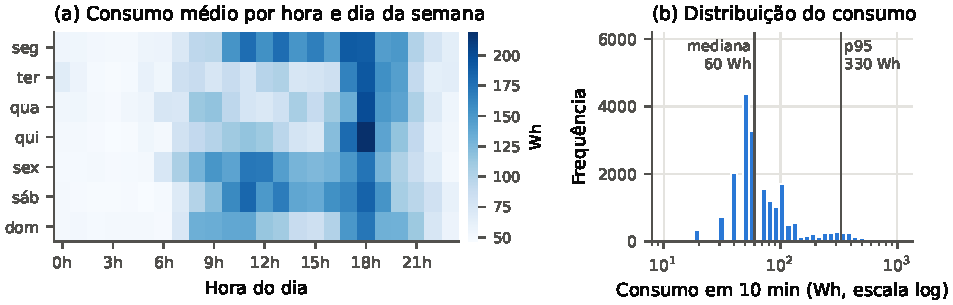
\includegraphics[width=\textwidth]{figures/fig1_eda}
  \caption{(a) Consumo médio dos eletrodomésticos por hora e dia da semana, na série completa. (b) Distribuição do consumo em escala logarítmica. Os valores são múltiplos de 10~Wh, o que explica as lacunas entre as barras.}
  \label{fig:eda}
\end{figure}

% ===========================================================================
\section{Pré-processamento e protocolo de avaliação}

\paragraph{Variáveis.} Renomeamos as colunas (por exemplo, \texttt{T1} vira \texttt{kitchen\_temp}) e removemos \texttt{rv1} e \texttt{rv2}. A hora do dia entra com codificação cíclica, $\sin(2\pi m/1440)$ e $\cos(2\pi m/1440)$ com $m$ em minutos, para que 23h50 fique próximo de 00h00. O dia da semana entra em \emph{one-hot}. As variáveis meteorológicas exigiram um cuidado: na base original, observações horárias foram interpoladas linearmente para 10 minutos, então o valor das 17h10 já contém parte da observação das 18h, ainda não disponível às 17h10. Para evitar esse vazamento, usamos em cada instante o valor da última hora cheia. Nas redes, o consumo entra em escala $\log(1+y)$, e o MLP recebe também a média móvel de 1~h e o desvio-padrão móvel de 6~h do consumo. Definimos ainda uma representação alternativa (\emph{variações}) para as 21 temperaturas e umidades: a variação em 10 e em 60 minutos e o desvio em relação à média das últimas 24~h, todas calculadas só com o passado.

\paragraph{Divisão temporal.} A divisão é cronológica, 70/15/15, com cortes à meia-noite. O treino vai de 11/01 a 15/04 (96 dias, 13\,716 linhas), a validação de 16/04 a 06/05 (21 dias, 3\,018) e o teste de 07/05 a 27/05 (21 dias, 2\,983). Preferimos 15\% de validação a 10\% porque o consumo médio semanal varia de cerca de 75 a 120~Wh, e duas semanas deixariam a seleção sensível a uma semana atípica. As respostas $y_{t+1}$ e $y_{t+6}$ são criadas dentro de cada conjunto, de modo que nenhum valor de validação ou teste é usado como resposta no treino.

\paragraph{Prevenção de vazamento.} Além da correção do clima, adotamos as seguintes medidas:
\begin{itemize}\setlength\itemsep{0pt}
  \item a padronização (\texttt{StandardScaler}) é ajustada só nas linhas de treino e reajustada em cada dobra da validação temporal;
  \item a ACF e a PACF, usadas para escolher as defasagens do ARX, são calculadas só no treino;
  \item as defasagens e janelas são construídas sobre a série contínua e só depois separadas por conjunto. Uma origem de teste pode usar o histórico do fim da validação, informação que existiria em produção, e todos os modelos são avaliados exatamente nas mesmas origens;
  \item hiperparâmetros e parada antecipada usam a validação, nunca o teste.
\end{itemize}

\paragraph{Métricas.} Reportamos MAE e RMSE em Wh e o MASE \citep{hyndman2006}, a razão entre o MAE do modelo e o MAE da persistência no treino para o mesmo horizonte (30,8 e 60,3~Wh). Para as redes, reportamos média e desvio-padrão entre cinco sementes. Também analisamos o erro por hora do dia e a autocorrelação dos resíduos com o teste de Ljung--Box \citep{ljungbox1978}, usando origens espaçadas pelo horizonte.

\paragraph{Seleção de modelos: dois protocolos.} Na rodada~1, os hiperparâmetros foram escolhidos pelo MAE na validação. Depois do resultado de teste da rodada~1 (Seção~\ref{sec:r1}), passamos a escolher entre alternativas com uma validação com janelas expansivas (\emph{forward chaining}) \citep{tashman2000,bergmeir2012}, sem tocar no teste. O período de treino e validação foi dividido em três blocos de avaliação de 21 dias (Figura~\ref{fig:protocolo}), e o último é a validação oficial. Em cada dobra, o treino é tudo o que vem antes do bloco, as padronizações são reajustadas e as redes usam os últimos 7 dias do treino da dobra para a parada antecipada. As regras de decisão foram escritas antes de rodar as dobras: vence a alternativa com o menor MASE médio entre dobras e horizontes.

\begin{figure}[t]
  \centering
  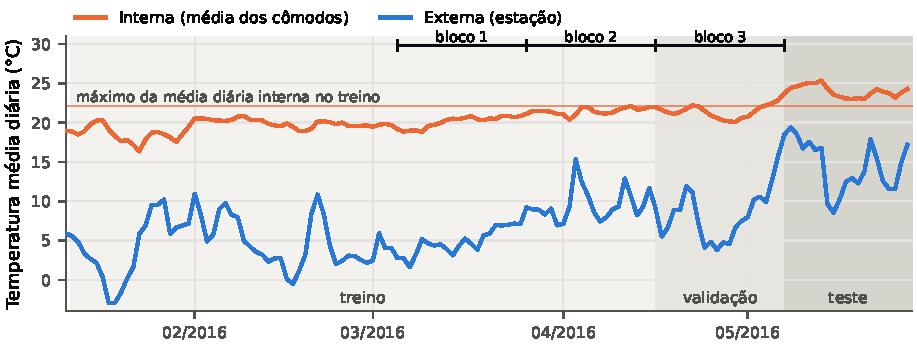
\includegraphics[width=\textwidth]{figures/fig2_protocolo}
  \caption{Temperatura média diária interna e externa, com a divisão em treino, validação e teste e os três blocos de avaliação da validação com janelas expansivas. No teste, a temperatura interna fica quase todo o tempo acima do máximo visto no treino.}
  \label{fig:protocolo}
\end{figure}

% ===========================================================================
\section{Modelos}

\paragraph{Persistência.} $\hat y_{t+h} = y_t$. É a referência do MASE e é difícil de bater a 10 minutos.

\paragraph{ARX.} Para cada horizonte ajustamos uma regressão Ridge separada (estratégia direta):
\begin{equation*}
\hat y_{t+h} = c + \sum_{i=0}^{p-1}\phi_i\, y_{t-i} + \sum_{j=0}^{q}\beta_j^\top x_{t-j} + \gamma^\top z_t + \delta\, y_{t+h-144},
\end{equation*}
em que $x$ são as variáveis medidas, $z$ o calendário e o último termo o consumo no mesmo horário do dia anterior (opcional). As entradas são padronizadas e a resposta fica em Wh, já que o Ridge é invariante à escala da resposta. Na validação foram escolhidos $p=12$ (sugerido pela PACF), $q=0$, a defasagem de 24~h e $\alpha = 100$ e $1000$ para 10 e 60 minutos.

\paragraph{MLP.} Recebe 49 variáveis: os 12 últimos consumos em $\log(1+y)$, as estatísticas móveis, os sensores, o clima e o calendário. Tem duas camadas ocultas de 128 neurônios com ReLU e dropout de 0,2, e prevê os seis passos à frente ($t+1, \dots, t+6$) em escala $\log(1+y)$. O treino usa a perda de Huber, AdamW (taxa $10^{-3}$, lotes de 256) e parada antecipada com paciência de 15 épocas. A janela ($L \in \{6, 12, 36\}$), a largura, o dropout e a taxa foram escolhidos na validação.

\paragraph{CNN 1D.} Recebe uma janela de $L=6$ passos com 36 canais (consumo, sensores, clima e calendário). Aplica duas convoluções temporais (32 filtros, kernel 3, ReLU) e uma camada linear, com dropout de 0,2, que produz as seis saídas. O treino é o mesmo do MLP, com taxa de $3\times 10^{-4}$.

\paragraph{Cabeça residual e variantes da rodada~2.} A rodada~1 mostrou que as redes que preveem o \emph{nível} do consumo extrapolam mal fora da faixa de treino (Seção~\ref{sec:r1}). Uma auditoria da comparação apontou também que o ARX usava a defasagem de 24~h, que as redes não recebiam. Testamos então duas mudanças. A primeira é uma \emph{cabeça residual}: a rede $f$ prevê a variação em relação ao consumo atual,
\begin{equation*}
\log(1+\hat y_{t+k}) = \log(1+y_t) + f_k(\mathbf{x}_t),
\end{equation*}
e assim parte da persistência, o que limita o efeito de extrapolações. A segunda é a defasagem de 24~h como entrada. Testamos também um \emph{ARX + MLP}, em que um MLP prevê o erro do ARX. Os resíduos de treino desse MLP são fora da amostra, vindos de reajustes mensais do ARX com janela expansiva, porque os resíduos dentro da amostra subestimariam o erro real.

\paragraph{GRU.} O modelo principal é uma GRU \citep{cho2014} unidirecional. Ela recebe uma janela de $L$ passos com 30 variáveis (consumo em $\log(1+y)$, luzes, sensores, clima e seno e cosseno da hora e do dia da semana). O último estado oculto é concatenado ao calendário dos instantes previstos e passa por uma camada linear com cabeça residual. O treino usa a perda L1, coerente com o MAE, \emph{clipping} do gradiente em 1,0 e AdamW. A busca em grade cobriu $L \in \{36, 72, 144\}$ (6, 12 e 24~h), estado oculto de 32, 64 ou 128, 1 ou 2 camadas e dropout de 0,1 ou 0,2, num total de 36 configurações. A escolhida tem $L=72$, duas camadas de 128 e dropout de 0,1. A busca foi pouco sensível: as 10 melhores configurações ficaram a menos de 0,5~Wh umas das outras na média dos dois horizontes. Um único modelo para os dois horizontes foi melhor que modelos separados (29,8 contra 30,1~Wh na validação). Como ablação, treinamos uma LSTM \citep{hochreiter1997} com a mesma configuração. A Tabela~\ref{tab:modelos} resume os modelos e seu custo.

\begin{table}[t]
  \centering\small
  \caption{Configurações finais e custo computacional (média de 5 sementes; GRU e LSTM em GPU, as demais redes em CPU). Inferência: uma passagem pelas 2\,983 origens do teste.}
  \label{tab:modelos}
  \begin{tabular}{@{}lp{4.6cm}p{3.6cm}rrr@{}}
\toprule
Modelo & Entrada & Arquitetura & Parâm. & Treino (s) & Inf. (ms) \\
\midrule
ARX (Ridge) & defasagens $y_{t-11..t}$, $y_{t+h-144}$, exógenas em $t$ & linear, um modelo por horizonte & --- & --- & --- \\
MLP & 49 variáveis (12 defasagens em $\log(1+y)$, estat. móveis, sensores, calendário) & 2 camadas ocultas de 128, dropout 0,2 & 23\,686 & 7,3 & 1,0 \\
CNN 1D & janela de 6 passos $\times$ 36 canais & 2 conv.\ (32 filtros, kernel 3), dropout 0,2 & 7\,750 & 8,3 & 2,0 \\
ARX + MLP & entradas do MLP + previsões do ARX & MLP sobre os resíduos do ARX (perda L1) & 23\,426 & 7,7 & 0,9 \\
GRU & janela de 72 passos (12 h) $\times$ 30 variáveis + calendário do alvo & 2 camadas de 128, dropout 0,1 & 160\,786 & 10,0 & 22,9 \\
LSTM & idem GRU & idem GRU & 214\,290 & 11,5 & 28,7 \\
\bottomrule
\end{tabular}

\end{table}

% ===========================================================================
\section{Resultados}

\subsection{Rodada 1: bom na validação, ruim no teste}\label{sec:r1}

Na validação, o MLP empatou com a persistência a 10 minutos e superou o ARX a 60 minutos (38,1 contra 42,9~Wh; Tabela~\ref{tab:resultados}). No teste, as duas redes ficaram atrás da persistência e do ARX, com grande variação entre sementes. O resíduo médio foi negativo, ou seja, as redes superestimaram o consumo: $-11$ e $-16$~Wh para o MLP e $-63$ e $-64$~Wh para a CNN 1D, enquanto o ARX e a persistência ficaram praticamente sem viés. A causa mais provável é a mudança na distribuição das entradas \citep{quinonero2009}. Padronizada com as estatísticas de treino, a temperatura da cozinha tem média de 0,75 na validação e 2,55 no teste, enquanto a distribuição do consumo pouco muda entre os conjuntos. Fora da faixa de treino, cada rede com ReLU extrapola de um jeito, o que também explica a variação entre sementes. O ARX, linear e com coeficientes encolhidos, extrapola de forma mais contida.

\begin{table}[t]
  \centering\small
  \caption{MAE (Wh) em treino, validação e teste e RMSE (Wh) no teste, para os horizontes de 10 e 60 minutos. Redes: média de 5 sementes, com o desvio-padrão do teste entre parênteses. ``---'': valor não registrado na execução final do notebook.}
  \label{tab:resultados}
  \begin{tabular}{@{}lcccccccc@{}}
\toprule
 & \multicolumn{2}{c}{MAE treino} & \multicolumn{2}{c}{MAE validação} & \multicolumn{2}{c}{MAE teste} & \multicolumn{2}{c}{RMSE teste} \\
\cmidrule(lr){2-3}\cmidrule(lr){4-5}\cmidrule(lr){6-7}\cmidrule(l){8-9}
Modelo & 10 & 60 & 10 & 60 & 10 & 60 & 10 & 60 \\
\midrule
\multicolumn{9}{@{}l}{\emph{Rodada 1}} \\
Persistência & 30,8 & 60,3 & 26,8 & 53,3 & 26,5 & 46,0 & 66,5 & 101,3 \\
ARX & 31,6 & 50,1 & 27,4 & 42,9 & 27,1 & 40,3 & 59,4 & 78,4 \\
MLP & 28,9 & 40,4 & 26,8 & 38,1 & 36,5 (3,3) & 52,4 (5,6) & 66,1 & 86,4 \\
CNN 1D & 33,8 & 41,6 & 35,0 & 43,1 & 83,6 (18,5) & 91,1 (11,7) & 122,1 & 130,2 \\
\multicolumn{9}{@{}l}{\emph{Rodada 2}} \\
MLP (residual) & --- & --- & 24,6 & 37,6 & 24,2 (0,2) & 35,4 (0,8) & 60,1 & 81,1 \\
CNN 1D (residual) & --- & --- & --- & --- & 25,0 (0,2) & 37,3 (0,8) & 60,9 & 83,1 \\
ARX + MLP & 25,9 & 35,2 & 25,2 & 38,1 & 24,6 (0,4) & 35,5 (0,8) & 59,3 & 81,7 \\
LSTM & 27,8 & 39,4 & 24,6 & 36,7 & 24,2 (0,1) & 35,4 (1,2) & 61,1 & 83,7 \\
\textbf{GRU} & 27,7 & 40,8 & 24,3 & 36,3 & 23,7 (0,3) & 35,0 (0,8) & 60,6 & 81,1 \\
\bottomrule
\end{tabular}

\end{table}

\subsection{Validação com janelas expansivas}

Antes das dobras, o teste KPSS \citep{kpss1992} no treino rejeitou a estacionariedade das 21 temperaturas e umidades em nível e de nenhuma de suas variações horárias. Isso motivou a comparação entre as representações \emph{níveis} e \emph{variações}, feita com o ARX e o MLP e com os hiperparâmetros da rodada~1 (Tabela~\ref{tab:dobras}). A regra escolheu \emph{níveis} (MASE médio de 0,905 contra 1,154): com \emph{variações}, o ARX piorou levemente e o MLP ficou instável na dobra~2. O resultado tem uma ressalva. Dentro do período de treino e validação, a mudança de distribuição é pequena: só 5\% a 10\% dos valores em nível de cada bloco ficam fora da faixa (quantis de 0,5\% a 99,5\%) do treino da dobra. As dobras, portanto, premiam pouco a robustez a essa mudança.

Nas mesmas dobras, a cabeça residual foi a mudança decisiva. O MASE médio caiu de 0,971 para 0,770 no MLP e de 1,454 para 0,792 na CNN 1D, nas três dobras e nos dois horizontes. A defasagem de 24~h praticamente não alterou o resultado. O ARX + MLP reduziu o MASE do ARX de 0,841 para 0,831 e foi considerado útil pela regra.

\begin{table}[t]
  \centering\small
  \caption{MASE médio nas três dobras da validação com janelas expansivas (menor é melhor). Em negrito, as alternativas escolhidas pelas regras fixadas antes de rodar as dobras.}
  \label{tab:dobras}
  \begin{tabular}{@{}llccc@{}}
\toprule
Decisão & Configuração & 10 min & 60 min & Média \\
\midrule
Representação & ARX, níveis & 0,945 & 0,735 & 0,840 \\
Representação & MLP, níveis & 1,136 & 0,805 & 0,971 \\
Representação & ARX, variações & 0,970 & 0,772 & 0,871 \\
Representação & MLP, variações & 1,528 & 1,345 & 1,436 \\
\addlinespace
Variante & MLP & 1,136 & 0,805 & 0,970 \\
Variante & MLP (24 h) & 1,173 & 0,796 & 0,985 \\
Variante & MLP (residual) & 0,863 & 0,677 & \textbf{0,770} \\
Variante & MLP (residual + 24 h) & 0,864 & 0,680 & 0,772 \\
Variante & CNN 1D & 1,860 & 1,048 & 1,454 \\
Variante & CNN 1D (24 h) & 1,772 & 1,011 & 1,391 \\
Variante & CNN 1D (residual) & 0,878 & 0,705 & \textbf{0,791} \\
Variante & CNN 1D (residual + 24 h) & 0,882 & 0,704 & 0,793 \\
\addlinespace
Correção do ARX & ARX & 0,945 & 0,735 & 0,840 \\
Correção do ARX & ARX + MLP & 0,919 & 0,742 & \textbf{0,831} \\
\bottomrule
\end{tabular}

\end{table}

\subsection{Comparação final}

Com a cabeça residual, as redes passaram do último para o primeiro lugar (Tabela~\ref{tab:resultados}). A GRU teve o menor MAE de teste nos dois horizontes: 23,7 e 35,0~Wh, ou MASE de 0,77 e 0,58. Em relação ao ARX, o MAE caiu 12\% e 13\%, e em relação à persistência, 11\% e 24\%. A vantagem da GRU sobre o MLP residual, porém, é de apenas 0,5 e 0,3~Wh, da ordem da variação entre sementes: a maior parte do ganho vem da cabeça residual, e não da arquitetura recorrente. O desvio-padrão entre sementes caiu de 3,3~Wh (MLP da rodada~1, 10 minutos) para 0,1 a 0,8~Wh, e o MAE de teste ficou próximo do de validação, o que indica que a âncora na persistência neutralizou a mudança de distribuição.\footnote{A GRU e a LSTM variam levemente entre execuções em GPU, mesmo com o cuDNN em modo determinístico; numa execução anterior, a GRU teve 23,6 e 34,9~Wh. A diferença é menor que a variação entre sementes.}

Em RMSE, o ARX continua competitivo (59,4 e 78,4~Wh, contra 60,6 e 81,1~Wh da GRU), o que já indica erros maiores das redes nos picos. A Figura~\ref{fig:hora} mostra que o erro se concentra no pico da manhã e às 17--18h, e que a GRU fica abaixo do ARX na maior parte das horas. O teste de Ljung--Box rejeita a ausência de autocorrelação dos resíduos a 10 minutos para todos os modelos, de modo que ainda há estrutura não capturada. As redes residuais subestimam o consumo em média (resíduo médio de $+5{,}8$ e $+12{,}5$~Wh para a GRU). A GRU é também a mais cara: 161 mil parâmetros e 23~ms de inferência no teste, contra 24 mil e 1~ms do MLP.

\begin{figure}[t]
  \centering
  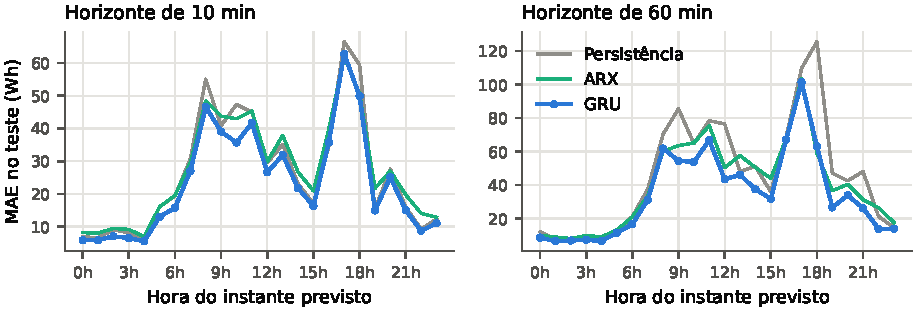
\includegraphics[width=\textwidth]{figures/fig3_mae_hora}
  \caption{MAE no teste por hora do instante previsto (GRU: média de 5 sementes).}
  \label{fig:hora}
\end{figure}

% ===========================================================================
\section{Extra: um modelo de fundação (Chronos-2)}

Como complemento, fora da comparação principal, avaliamos o Chronos-2 \citep{chronos2}. É um \emph{transformer} pré-treinado para séries temporais, com cerca de 120 milhões de parâmetros, que prevê quantis e aceita covariáveis. Usamos as mesmas origens de teste dos outros modelos, o alvo em Wh, o calendário como covariável conhecida no futuro e os sensores e o clima como covariáveis só do passado. Cada origem foi prevista isoladamente, para que uma janela não visse outras posteriores. Testamos o modelo sem ajuste (\emph{zero-shot}) e com ajuste fino por LoRA \citep{hu2022} ($r=8$, $\alpha=16$). No ajuste, as janelas de treino vieram só do período de treino, e a taxa de aprendizado e o \emph{checkpoint} foram escolhidos pela perda quantílica (WQL) na validação. Não encontramos a base nos corpora públicos de pré-treinamento (\texttt{chronos\_datasets} e GIFT-Eval; \citealp{gifteval2024}).

Com 12~h de contexto, o Chronos-2 empata com a persistência. Com 7 dias de contexto, sem nenhum treino nesta casa, atinge o nível da GRU (Tabela~\ref{tab:chronos}). O LoRA traz um ganho modesto e o menor MAE do trabalho a 60 minutos (33,3~Wh, 1,8~Wh abaixo da GRU), com intervalos de 80\% bem calibrados (79\% de cobertura). O clima futuro não ajuda. A comparação não é justa: o modelo tem 120 milhões de parâmetros contra 161 mil, foi pré-treinado em um grande corpus, usa 7 dias de contexto contra 12~h, foi treinado com uma única semente e levou cerca de 50 minutos de GPU por taxa de aprendizado.

\begin{table}[t]
  \centering\small
  \caption{Chronos-2 no teste: MAE da mediana, cobertura do intervalo entre os quantis 0,1 e 0,9 (nominal de 80\%) e WQL. $^\dagger$Limite superior irreal: supõe o clima futuro conhecido.}
  \label{tab:chronos}
  \begin{tabular}{@{}lcccccc@{}}
\toprule
 & \multicolumn{2}{c}{MAE (Wh)} & \multicolumn{2}{c}{Cobertura 80\%} & \multicolumn{2}{c}{WQL} \\
\cmidrule(lr){2-3}\cmidrule(lr){4-5}\cmidrule(l){6-7}
Chronos-2 & 10 & 60 & 10 & 60 & 10 & 60 \\
\midrule
Zero-shot, 12 h & 26,5 & 41,1 & 78\% & 76\% & 0,231 & 0,365 \\
Zero-shot, 7 dias & 24,0 & 34,5 & 76\% & 78\% & 0,209 & 0,302 \\
LoRA, 7 dias & 23,6 & 33,3 & 79\% & 79\% & 0,204 & 0,287 \\
Zero-shot, 7 dias + clima futuro$^\dagger$ & 24,2 & 34,5 & 77\% & 78\% & 0,210 & 0,302 \\
\bottomrule
\end{tabular}

\end{table}

% ===========================================================================
\section{Quando o modelo de aprendizagem profunda falha?}\label{sec:falha}

\paragraph{Mudança na distribuição das entradas.} As redes que preveem o nível do consumo falham quando as entradas saem da faixa de treino, e a validação feita com dados do passado não reproduz essa situação. Nas nossas dobras, só 5\% a 10\% dos valores ficavam fora da faixa, contra quase todo o teste (Figura~\ref{fig:protocolo}). Por isso a troca de representação não se validou, embora atacasse justamente o problema. A cabeça residual mitiga a falha, mas não faz a rede entender a relação entre temperatura e consumo: um mês de verão, ainda mais quente, poderia afetar novamente as variáveis exógenas. Uma série que cubra pelo menos um ano evitaria essa extrapolação.

\paragraph{Picos de consumo.} O ganho das redes vem das leituras comuns. No teste a 60 minutos, nas leituras de até 300~Wh (95,7\% das observações), o MAE é de 22,0~Wh para a GRU, contra 28,6~Wh do ARX e 34,7~Wh da persistência. Nas leituras acima de 300~Wh (4,3\%), a GRU erra mais que os dois: 321~Wh, contra 296~Wh do ARX e da persistência. O Chronos-2 com LoRA segue o mesmo padrão, com o menor erro nas leituras comuns (19,6~Wh) e o maior nos picos (334~Wh). As perdas L1 e Huber sobre $\log(1+y)$ aproximam a mediana condicional, que não antecipa um evento raro e abrupto. A Figura~\ref{fig:dia} mostra o efeito: nenhum modelo prevê o pico das 18h, e a GRU só reage uma hora depois, quando o pico já passou. Prever esses picos, que respondem por boa parte do RMSE, exigiria outra formulação, como perdas quantílicas, um classificador de eventos ou informação sobre o uso dos aparelhos.

\begin{figure}[t]
  \centering
  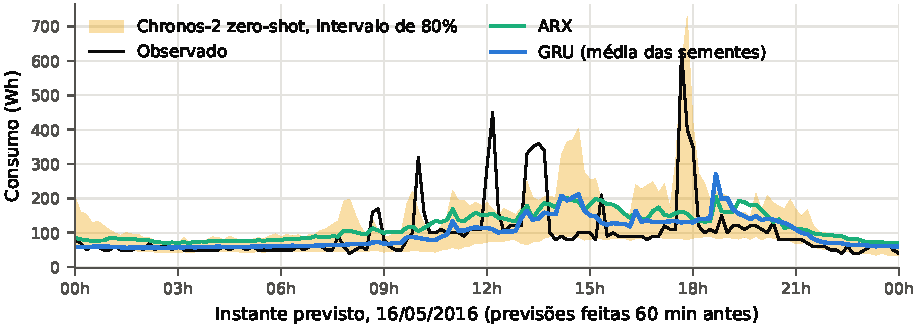
\includegraphics[width=\textwidth]{figures/fig4_dia_teste}
  \caption{Um dia do teste, horizonte de 60 minutos: consumo observado, previsões da GRU (média de 5 sementes) e do ARX e intervalo de 80\% do Chronos-2 \emph{zero-shot} com 7 dias de contexto. Os picos só aparecem nas previsões depois de terem ocorrido.}
  \label{fig:dia}
\end{figure}

\paragraph{Riscos de vazamento remanescentes.} Algumas escolhas usaram informação do teste de forma indireta, e as listamos para que os números sejam lidos com a devida cautela:
\begin{itemize}\setlength\itemsep{0pt}
  \item a análise exploratória usou a série completa, incluindo o teste, e foi ela que revelou a tendência sazonal;
  \item a rodada~2 (cabeça residual, defasagem de 24~h, ARX + MLP) e a GRU foram desenvolvidas depois de vermos o resultado de teste da rodada~1. As escolhas foram feitas por regras fixadas antes, em dobras que não tocam o teste, mas a decisão de procurar uma correção foi motivada pelo teste. Os resultados de teste da rodada~2 devem, portanto, ser lidos como levemente otimistas;
  \item o teste cobre só três semanas de uma única casa, e as diferenças de menos de 1~Wh entre as redes residuais estão dentro da variação entre sementes.
\end{itemize}

\paragraph{Conclusão.} Em previsão de curtíssimo prazo, a persistência é uma referência forte, e a escolha mais importante foi ancorar as redes nela. Com a cabeça residual, todas as redes superaram a persistência e o ARX, e a GRU foi a melhor, por pouco. Os limites estão na mudança de distribuição, que só uma série mais longa resolveria, e nos picos de consumo, que nenhum dos modelos, incluindo um modelo de fundação, antecipa. O bom desempenho do Chronos-2 com uma semana de contexto e nenhum treino nesta casa sugere que ele deveria entrar como referência em comparações futuras.

\bibliographystyle{plainnat}
\bibliography{refs}

\end{document}
